\chapter{Batch Python Scripting}
\label{chap:BatchPythonScripting}

\index{Python|(}

Python scripting can be leveraged in two ways within ParaView.  First,
Python scripts can automate the setup and execution of visualizations by
performing the same actions as a user at the GUI.  Second, Python scripts
can be run inside pipeline objects, thereby performing parallel
visualization algorithms.  This chapter describes the first mode, batch
scripting for automating the visualization.

Batch scripting is a good way to automate mundane or repetitive tasks, but
it is also a critical component when using ParaView in situations where the
GUI is undesired or unavailable.  The automation of Python scripts allows
you to leverage ParaView as a scalable parallel post-processing framework.
We are also leveraging Python scripting to establish \emph{in situ}
computation within simulation code. (ParaView supports an \emph{in situ}
library called \index{Catalyst}\keyterm{Catalyst}, which is not documented
in this tutorial.  See
\href{http://catalyst.paraview.org/}{http://catalyst.paraview.org/} for
more information on Catalyst).

This tutorial gives only a brief introduction to Python scripting. More
comprehensive documentation on scripting is given in the \emph{ParaView
  User's Guide}. There are also further links on ParaView's documentation
web page
(\href{http://www.paraview.org/documentation}{http://www.paraview.org/documentation})
including a complete reference to the ParaView Python API.

\section{Starting the Python Interpreter}
\label{sec:StartingThePythonInterpreter}

There are many ways to invoke the Python interpreter.  The method you use
depends on how you are using the scripting.  The easiest way to get a
python interpreter, and the method we use in this tutorial, is to select
\gui{Tools} \ra \gui{Python Shell} from the menu.  This will bring up a
dialog box containing controls for ParaView's Python shell. This is the 
Python interpreter, where you directly control
ParaView via the interface described below. 

\begin{inlinefig}
  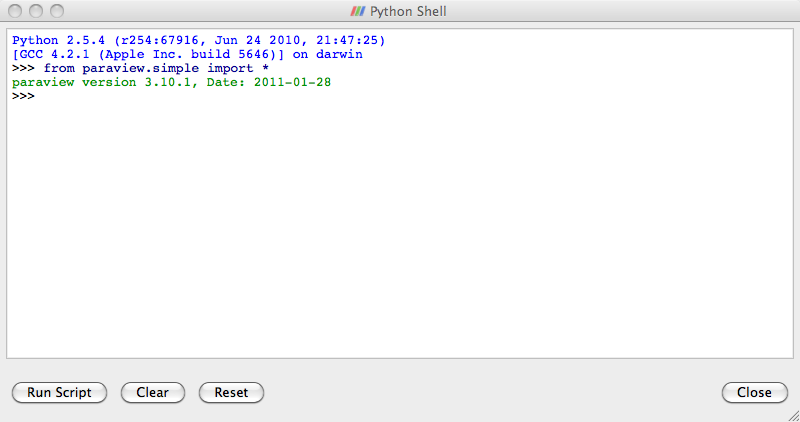
\includegraphics[width=\scw]{images/PythonShellDialog}
\end{inlinefig}

If you are most interested in getting started on writing scripts,
feel free to skip to the next section past the discussion of the other ways
to invoke scripting.

ParaView comes with two command line programs that execute Python scripts:
\progname{pvpython} and \progname{pvbatch}.  They are similar to the
\progname{python} executable that comes with Python distributions in
that they accept Python scripts either from the command line or from a file
and they feed the scripts to the Python interpreter.

The difference between \progname{pvpython} and \progname{pvbatch} is
subtle and has to do with the way they establish the visualization
service.  \progname{pvpython} is roughly equivalent to the
\progname{paraview} client GUI with the GUI replaced with the Python
interpreter.  It is a serial application that connects to a ParaView server
(which can be either builtin or remote).  \progname{pvbatch} is roughly
equivalent to \progname{pvserver} except that commands are taken from a
Python script rather than from a socket connection to a ParaView client.  
It is a
parallel application that can be launched with \progname{mpirun} (assuming
it was compiled with MPI), but it cannot connect to another server; it is
its own server.  In general, you should use \progname{pvpython} if you
will be using the interpreter interactively and \progname{pvbatch} if
you are running in parallel.

It is also possible to use the ParaView Python modules from programs
outside of ParaView.  This can be done by pointing the \texttt{PYTHONPATH}
environment variable to the location of the ParaView libraries and Python
modules and pointing the \texttt{LD\_LIBRARY\_PATH} (on Unix/Linux),
\texttt{DYLD\_LIBRARY\_PATH} (on Mac), or \texttt{PATH} (on Windows)
environment variable to the ParaView libraries.  Running the Python script
this way allows you to take advantage of third-party applications such as
IDLE.  For more information on setting up your environment, consult the
ParaView Wiki.

\section{Tracing ParaView State}
\label{sec:TracingParaViewState}

\index{Python!trace|(}

Before diving into the depths of the Python scripting features, let us take
a moment to explore the automated facilities for creating Python scripts.
The ParaView GUI's Python \gui{Trace}\index{trace} feature allows one to
very easily create Python scripts for many common tasks. To use
\gui{Trace}, one simply begins a trace recording via \gui{Start Trace},
found in the \gui{Tools} menu, and ends a trace recording via \gui{Stop Trace},
also found in the \gui{Tools} menu. This produces a Python script that
reconstructs the actions taken in the GUI. That script contains the same
set of operations that we are about to describe. As such, \gui{Trace}
recordings are a good resource when you are trying to figure out how to do
some action via the Python interface, and conversely the following
descriptions will help in understanding the contents of any given
\gui{Trace} script.

\begin{exercise}{Creating a Python Script Trace}
  \label{ex:CreatingAPythonScriptTrace}%
  If you have been following an exercise in a previous section, now is a
  good time to reset ParaView.  The easiest way to do this is to select
  \gui{Edit} \ra \gui{Reset Session} from the menu.

  \begin{enumerate}
  \item Click the \gui{Start Trace} in the \gui{Tools} menu.
  \item A dialog box with options for the trace is presented. We will
    discuss the meaning of these options later. For now, just click
    \gui{OK}.
  \item Build a simple pipeline in the main
    ParaView GUI.  For example, create a sphere source and then clip it.
  \item Click \gui{Stop Trace} in the \gui{Tools} menu.
  \item An editing window will open populated with a Python script that
    replicates the operations you just made.
    %% Save the Python script to somewhere on your hard drive.
  \end{enumerate}

  Even if you have not been exposed to ParaView's Python bindings, the
  commands being performed in the traced script should be familiar.  Once
  saved to your hard drive, you can of course edit the script with your
  favorite editor.  The final script can be interpreted by the
  \progname{pvpython} or \progname{pvbatch} program for totally
  automated visualization.  It is also possible to run this script in the
  GUI.  The \gui{Python Shell} dialog has a \gui{Run Script} button that
  invokes a saved script.
\end{exercise}

It should be noted that there is also a way to capture the current ParaView
state as a Python script without tracing actions.  Simply select \gui{Save
  State...} from the ParaView \gui{File} menu and choose to save as a
Python .py state file (as opposed to a ParaView .pvsm state file).  We will
not have an exercise on state Python scripts, but suffice it to say they
can be used in much the same way as traced Python scripts.  You are welcome
to experiment with this feature as you like.

\begin{inlinefig}
  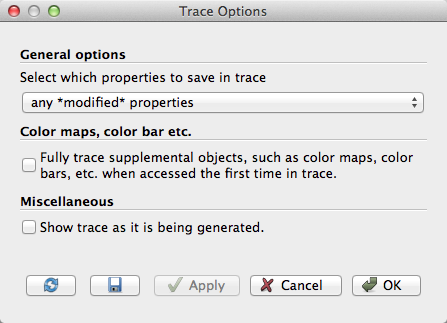
\includegraphics[width=0.8\scw]{images/TraceOptions}
\end{inlinefig}

As noted earlier in the exercise, Python tracing has some options that are
presented in a dialog box before the tracing starts. The first option
selections what properties are saved to the trace. Some properties you
explicitly set through the GUI, such as a value entered in a GUI
widget. Some properties are set internally by the ParaView application,
such as the initial position of a clip plane based on the bounds of the
object it is being applied to. Many other properties are left at some
default value. You can choose one of the following classes of properties to
save:
\begin{description}
\item[\gui{all properties}] Traces the values of all properties even if
  they remain at the default. This can be helpful to introspect all
  possible properties or to ensure a consistent state regardless of the
  settings for other users. This also yields a very verbose output that can
  be hard to read.
\item[\gui{any *modified* properties}] Ignores any properties that do not
  change from their defaults. This is a good option for most use cases.
\item[\gui{only *user-modified* properties}] Ignores any properties that
  are not explicitly set by the user. Traces of this nature rely on any
  internally set properties being reapplied when the script is run.
\end{description}

The next option has to do with supplemental objects that are managed by the
ParaView GUI (or client) rather than in the server's state. Check this box
to capture all of the state associated with these objects, which includes
color maps, color bars, and other annotation.

Finally, ParaView provides the option to show the trace file as it is being
generated. This can be a helpful option to use when learning what Python
commands can be used to replicate particular actions in the ParaView GUI.

\index{Python!trace|)}

\section{Macros}
\label{sec:Macros}

\index{macro|(}
\index{Python!macro|(}

A simple but powerful way to customize the behavior of ParaView is to
add your Python script as a \keyterm{macro}.  A macro is simply an 
automated script that can
be invoked through its button in a toolbar or its entry in the menu bar.
Any Python script can be assigned to a macro.

\begin{exercise}{Adding a Macro}
  \label{ex:AddingAMacro}%
  This exercise is a continuation of
  Exercise~\ref{ex:CreatingAPythonScriptTrace}.  You will need to finish
  that exercise before beginning this one.  You should have the editing
  window containing the Python script created in
  Exercise~\ref{ex:CreatingAPythonScriptTrace} open.

  \begin{enumerate}
  \item In the menu bar (of the editing window), select \gui{File} \ra
    \gui{Save As Macro...}.
  \item Choose a descriptive name for the macro file and save it in the
    default directory provided by the browser.  You should now see 
    your macro on the Macro toolbar at the top of the ParaView GUI.
    \savecounter
  \end{enumerate}

  At this point, you should now see your macro added to the toolbars.  By
  default, macro toolbar buttons are placed in the middle row all the way
  to the left.  If you are short on space in your GUI, you may need to move
  toolbars around to see it.  You will also see that your macro has been
  added to the \gui{Macros} menu.

  \begin{enumerate}
    \restorecounter
  \item Close the Python editor window.
  \item Delete the pipeline you have created by either selecting \gui{Edit}
    \ra \gui{Delete All} from the menu or selecting \gui{Edit} \ra
    \gui{Reset Session} from the menu.
  \item Activate your macro by clicking on the toolbar button or selecting
    it in the \gui{Macros} menu.
  \end{enumerate}

  In this example our macro created something from scratch.  This is
  helpful if you often load some data in the same way every time.  You can
  also trace the creation of filters that are applied to existing data.  A
  macro from a trace of this nature allows you to automate the same
  visualization on different data.
\end{exercise}

\index{macro|)}
\index{Python!macro|)}

\section{Creating a Pipeline}
\label{sec:CreatingAPipeline}

As described in the previous two sections, the ParaView GUI's Python
\gui{Trace} feature provides a simple mechanism to create scripts. In this
section we will begin to describe the basic bindings for ParaView
scripting. This is important information in building Python scripts, but
you can always fall back on producing traces with the GUI.

The first thing any ParaView Python script must do is load the
\textpy{paraview.simple} module.  This is done by invoking
\begin{python}
from paraview.simple import *
\end{python}
In general, this command needs to be invoked at the beginning of any
ParaView batch Python script.  This command is automatically invoked for
you when you bring up the scripting dialog in ParaView, but you must add it
yourself when using the Python interpreter in other programs (including
\progname{pvpython} and \progname{pvbatch}).

\index{proxy|seealso{Python, proxy}}

The \textpy{paraview.simple} module defines a function for every source,
reader, filter, and writer defined in ParaView.  The function will be the
same name as shown in the GUI menus with spaces and special characters
removed.  For example, the \pyfunc{Sphere} function corresponds to
\gui{Sources} \ra \gui{Sphere} in the GUI and the \pyfunc{PlotOverLine}
function corresponds to \gui{Filters} \ra \gui{Data Analysis} \ra \gui{Plot
  Over Line}.  Each function creates a pipeline object, which will show up
in the pipeline browser (with the exception of writers), and returns an
object that is a \keyterm{proxy}\index{Python!proxy} that can be used to
query and manipulate the properties of that pipeline object.

There are also several other functions in the \textpy{paraview.simple}
module that perform other manipulations.  For example, the pair of
functions \pyfunc{Show} and \pyfunc{Hide} turn on and off, respectively,
the visibility of a pipeline object in a view.  The \pyfunc{Render}
function causes a view to be redrawn.

To obtain a concise list of the functions available in \textpy{paraview.simple},
invoke \textpy{dir(paraview.simple)}. Alternatively, as explained in
Section~\ref{sec:OnlineHelp} you can get a verbose listing via
\textpy{help(paraview.simple)}.

\begin{exercise}{Creating and Showing a Source}
  \label{ex:CreatingAndShowingASource}%
  If you have been following an exercise in a previous section, now is a
  good time to reset ParaView.  The easiest way to do this is to select
  \gui{Edit} \ra \gui{Reset Session} from the menu.

  If you have not already done so, open the Python shell in the ParaView
  GUI by selecting \gui{Tools} \ra \gui{Python Shell} from the menu.  You
  will notice that
  \begin{python}
from paraview.simple import *
  \end{python}
  has been added for you.

  Create and show a \gui{Sphere} source by typing the following in the
  Python shell.
  \begin{python}
sphere = Sphere()
Show()
Render()
ResetCamera()
  \end{python}

  The \pyfunc{Sphere} command creates a sphere pipeline object.  Once it is
  executed you will see an item in the pipeline browser created.  We save a
  \index{Python!proxy}proxy to the pipeline object in the variable
  \textpy{sphere}.  We are not using this variable (yet), but it is good
  practice to save references to your pipeline objects.

  The subsequent \pyfunc{Show} command turns on visibility of this object
  in the view, and the subsequent \pyfunc{Render} causes the results to be
  seen. Finally, although the ParaView GUI automatically adjusts the camera
  to data shown for the first time, the Python scripting does not. The call
  to \pyfunc{ResetCamera} performs this automatic camera adjustment if
  necessary.

  At this point you can interact directly with the GUI again.  Try
  changing the camera angle in the view with the mouse.
\end{exercise}

\begin{exercise}{Creating and Showing a Filter}
  \label{ex:CreatingAndShowingAFilter}%
  Creating filters is almost identical to creating sources.  By default,
  the last created pipeline object will be set as the input to the newly
  created filter, much like when creating filters in the GUI.

  This exercise is a continuation of
  Exercise~\ref{ex:CreatingAndShowingASource}.  You will need to finish
  that exercise before beginning this one.

  Type in the following script in the Python shell that hides the sphere
  and then adds the shrink filter to the sphere and shows that.

  \pyfuncindex{Hide}\pyfuncindex{Show}\pyfuncindex{Shrink}\pyfuncindex{Render}
  \begin{python}
Hide()
shrink = Shrink()
Show()
Render()
  \end{python}

  The sphere should be replaced with the output of the \pyfunc{Shrink}
  filter, which makes all of the polygons smaller to give the mesh an
  exploded type of appearance.
\end{exercise}

So far as we have built pipelines we have accepted the default parameters
for the pipeline objects.  As we have seen in the exercises of
Chapter~\ref{chap:BasicUsage}, it is common to have to modify the
parameters of the objects using the properties panel.

In Python scripting, we use the \keyterm{proxy}\index{Python!proxy}
returned from the creation functions to manipulate the pipeline objects.
These proxies are in fact Python objects with class attributes that
correspond to the same properties you set in the properties panel.  They
have the same names as those in the properties panel with spaces and other
illegal characters removed.  Use \pyfunc{dir(variable)} or
\pyfunc{help(variable)} to get a list of all attributes on any variable
that you have access to.  In most cases, simply assign values to an object's
attributes in order to change them.

\begin{exercise}{Changing Pipeline Object Properties}
  \label{ex:ChangingPipelineObjectProperties}%
  This exercise is a continuation of Exercises
  \ref{ex:CreatingAndShowingASource} and
  \ref{ex:CreatingAndShowingAFilter}.  You will need to finish those
  exercises before beginning this one.

  Recall that we have so far created two Python variables, \textpy{sphere}
  and \textpy{shrink}, that are proxies to the corresponding pipeline
  objects.  First, enter the following command into the Python shell to get
  a concise listing of all attributes of the sphere.

  \begin{python}
dir(sphere)
  \end{python}

  Next, enter the following command into the Python shell to get
  the current value of the \gui{Theta Resolution} property of the sphere.

  \begin{python}
print sphere.ThetaResolution
  \end{python}

  The Python interpreter should respond with the result \textpy{8}.  (Note
  that using the \textpy{print} keyword, which instructs Python to output
  the arguments to standard out, is superfluous here as the Python shell
  will output the result of any command anyway.)  Let us double the number
  of polygons around the equator of the sphere by changing this property.

  \begin{python}
sphere.ThetaResolution = 16
Render()
  \end{python}

  The shrink filter has only one property, \gui{Shrink Factor}.  We can
  adjust this factor to make the size of the polygons larger or smaller.
  Let us change the factor to make the polygons smaller.

  \begin{python}
shrink.ShrinkFactor = 0.25
Render()
  \end{python}

  You may have noticed that as you type in Python commands to change the
  pipeline object properties, the GUI in the properties panel updates
  accordingly.
\end{exercise}

So far we have created only non-branching pipelines.  This is a simple and
common case and, like many other things in the \textpy{paraview.simple}
module, is designed to minimize the amount of work for the simple and
common case but also provide a clear path to the more complicated cases.
As we have built the non-branching pipeline, ParaView has automatically
connected the filter input to the previously created object so that the
script reads like the sequence of operations it is.  However, if the
pipeline has branching, we need to be more specific about the filter
inputs.

\begin{exercise}{Branching Pipelines}
  \label{ex:BranchingPipelines}%
  This exercise is a continuation of Exercises
  \ref{ex:CreatingAndShowingASource} through
  \ref{ex:ChangingPipelineObjectProperties}.  You will need to finish
  Exercises \ref{ex:CreatingAndShowingASource} and
  \ref{ex:CreatingAndShowingAFilter} before beginning this one
  (Exercise~\ref{ex:ChangingPipelineObjectProperties} is optional).

  Recall that we have so far created two Python variables, \textpy{sphere}
  and \textpy{shrink}, that are proxies to the corresponding pipeline
  objects.  We will now add a second filter to the sphere source that will
  extract the wireframe from it.  Enter the following in the Python shell.

  \pyfuncindex{ExtractEdges}
  \begin{python}
wireframe = ExtractEdges(Input=sphere)
Show()
Render()
  \end{python}

  An \gui{Extract Edges} filter is added to the sphere source.  You should
  now see both the wireframe of the original sphere and the shrunken
  polygons.

  Notice that we explicitly set the input for the \gui{Extract Edges}
  filter by providing \textpy{Input=sphere} as an argument to the
  \pyfunc{ExtractEdges} function.  What we are really doing is setting the
  \textpy{Input} property upon construction of the object.  Although it
  would be possible to create the object with the default input, and then
  set the input later, it is not recommended.  The problem is that not all
  filters accept all input.  If you initially create a filter with the
  wrong input, you could get error messages before you get a chance to
  change the \textpy{Input} property to the correct input.

  The sphere source having two filters connected to its output is an
  example of \keyterm{fan out} in the pipeline.  It is always possible to
  have multiple filters attached to a single output.  Some filters, but not
  all, also support having multiple filters connected to their input.
  Multiple filters are attached to an input is known as \keyterm{fan in}.
  In ParaView's Python scripting, fan in is handled much like fan out, by
  explicitly defining a filter's inputs.  When setting multiple inputs (on
  a single
  port\footnote{
  Filters that have multiple input ports, like \textpy{ResampleWithDataset},
  use different names to distinguish amongst the input properties instead.
  The ports are typically called
  ``Input'' and ``Source'' but consult \gui{Trace} or \pyfunc{help} to be sure.
  }), simply set the input to a list of pipeline objects rather
  than a single one.  For example, let us group the results of the shrink
  and extract edges filters using the \gui{Group Datasets} filter.  Type
  the following line in the Python shell.

  \pyfuncindex{GroupDatasets}
  \begin{python}
group = GroupDatasets(Input=[shrink,wireframe])
Show()
  \end{python}

  There is now no longer any reason for showing the shrink and extract
  edges filters, so let us hide them.  By default, the \pyfunc{Show} and
  \pyfunc{Hide} functions operate on the last pipeline object created (much
  like the default input when creating a filter), but you can explicitly
  choose the object by giving it as an argument.  To hide the shrink and
  extract edges filters, type the following in the Python shell.

  \begin{python}
Hide(shrink)
Hide(wireframe)
Render()
  \end{python}
\end{exercise}

In the previous exercise, we saw that we could set the \textpy{Input}
property by placing \textpy{Input=\argdesc{input object}} in the arguments
of the creator function.  In general we can set any of the properties at
object construction by specifying \textpy{\argdesc{property
    name}=\argdesc{property value}}.  For example, we can set both the
\gui{Theta Resolution} and \gui{Phi Resolution} when we create a sphere
with a line like this.

\begin{python}
sphere = Sphere(ThetaResolution=360, PhiResolution=180)
\end{python}


\section{Active Objects}
\label{sec:ActiveObjects}

If you have any experience with the ParaView GUI, then you should already
be familiar with the concept of an active object.  As you build and
manipulate visualizations within the GUI, you first have to select an
object in the pipeline browser.  Other GUI panels such as the properties
panel will change based on what the active object is.  The active
object is also used as the default object to use for some operations such
as adding a filter.

The batch Python scripting also understands the concept of the active
object.  In fact, when running together, the GUI and the Python interpreter
share the same active object.  When you created filters in the previous
section, the default input they were given was actually the active object.
When you created a new pipeline object, that new object became the active
one (just like when you create an object in the GUI).

You can get and set the active object with the \pyfunc{GetActiveSource} and
\pyfunc{SetActiveSource} functions, respectively.  You can also get a list
of all pipeline objects with the \pyfunc{GetSources} function.  When you
click on a new object in the GUI pipeline browser, the active object in
Python will change.  Likewise, if you call \pyfunc{SetActiveSource} in
python, you will see the corresponding entry become highlighted in the
pipeline browser.

\begin{exercise}{Experiment with Active Pipeline Objects}
  \label{ex:ExperimentWithActivePipelineObjects}%
  This exercise is a continuation of the exercises in the previous
  section.  However, if you prefer you can create any pipeline you want and
  follow along.

  Play with active objects by trying the following.
  \begin{itemize}
  \item Get a list of objects by calling
    \pyfuncindex{GetSources}\textpy{GetSources()}.  Find the sources and
    filters you created in that list.
  \item Get the active object by calling
    \pyfuncindex{GetActiveSource}\textpy{GetActiveSource()}.  Compare that
    to what is selected in the pipeline browser.
  \item Select something new in the pipeline browser and call
    \textpy{GetActiveSource()} again.
  \item Change the active object with the \textpy{SetActiveSource()}
    function. You can use one of the proxy objects you created earlier as
    an argument to \pyfunc{SetActiveSource}. Observe the change in the
    pipeline browser.
  \end{itemize}
\end{exercise}

In addition to maintaining an active pipeline object, ParaView Python
scripting also maintains an active view.  As a ParaView user, you should
also already be familiar with multiple views and the active view.  The
active view is marked in the GUI with a blue border.  The Python functions
\pyfunc{GetActiveView} and \pyfunc{SetActiveView} allow you to query and
change the active view.  As with pipeline objects, the active view is
synchronized between the GUI and the Python interpreter.


\section{Online Help}
\label{sec:OnlineHelp}

This tutorial, as well as similar instructions in the ParaView book and
Wiki, is designed to give the key concepts necessary to understand and
create batch Python scripts.  The detailed documentation including complete lists of
functions, classes, and properties available is maintained by the ParaView
build process and provided as online help from within the ParaView
application.  In this way we can ensure that the documentation is up to
date for whatever version of ParaView you are using and that it is easily
accessible.

The ParaView Python bindings make use of the \pyfunc{help} built-in
function.  This function takes as an argument any Python object and returns
some documentation on it.  For example, typing
\begin{python}
  help(paraview.simple)
\end{python}
returns a brief description of the module and then a list of all the
functions included in the module with a brief synopsis of what each one
does.  For example
\begin{python}
  help(Sphere)
  sphere = Sphere()
  help(sphere)
\end{python}
will first give help on the \pyfunc{Sphere} function, then use it to create
an object, and then give help on the object that was returned (including a
list of all the properties for the \index{Python!proxy}proxy).

Most of the widgets displayed in the properties panel's \gui{Properties} group
are automatically generated from the same introspection that builds the
Python classes. (There are a small number of exceptions where a custom
panel was created for better usability.) Thus, if you see a labeled widget
in the properties panel, there is a good chance that there is a
corresponding property in the Python object with the same name.

Regardless of whether the GUI contains a custom panel for a pipeline
object, you can still get information about that object's properties from
the GUI's online help.  As always, bring up the help with the
\icon{pqHelp32} toolbar button.  You can find documentation for all the
available pipeline objects under the \gui{Sources}, \gui{Filters},
\gui{Readers}, and \gui{Writers} entries in the help \gui{Contents}.  Each
entry gives a list of objects of that type.  Clicking on any one of the
objects gives a list of the properties you can set from within Python.

\begin{inlinefig}
  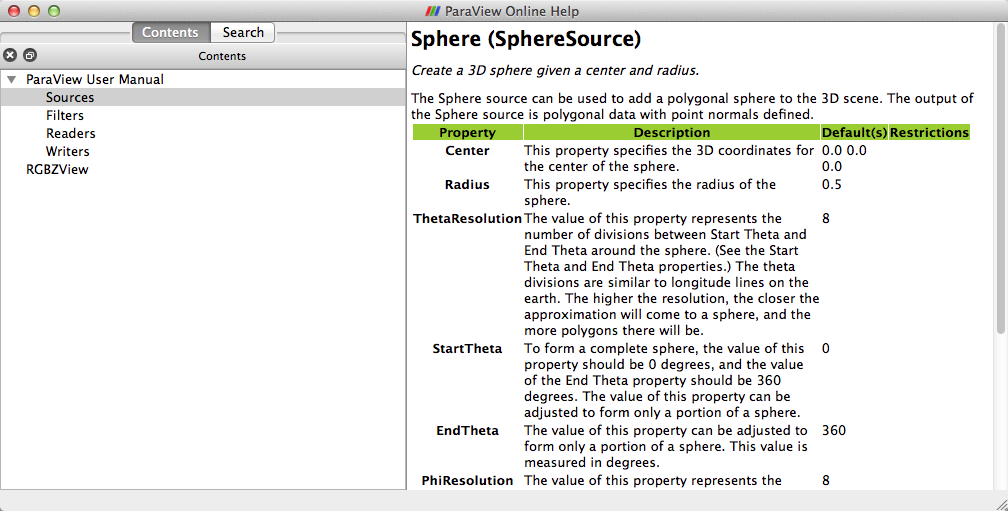
\includegraphics[width=\scw]{images/ObjectHelp}
\end{inlinefig}


\section{Reading from Files}
\label{sec:ReadingFromFiles}

The equivalent to opening a file in the ParaView GUI is to create a reader
in Python scripting.  Reader objects are created in much the same way as
sources and filters; \textpy{paraview.simple} has a function for each
reader type that creates the pipeline object and returns a
\index{Python!proxy}proxy object. One can instantiate any given reader
directly as described below, or more simply call \textpy{reader =
  OpenDataFile(\argdesc{filename})}

All reader objects have at least one property (hidden in the GUI) that
specifies the file name.  This property is conventionally called either
\textpy{FileName} or \textpy{FileNames}.  You should always specify a valid
file name when creating a reader by placing something like
\textpy{FileName=\argdesc{full path}} in the arguments of the construction
object.  Readers often do not initialize correctly if not given a valid
file name.

\begin{exercise}{Creating a Reader}
  \label{ex:CreatingAReader}%
  We are going to start a fresh visualization, so if you have been
  following along with the exercises so far, now is a good time to reset
  ParaView.  The easiest way to do this is to select \gui{Edit} \ra
  \gui{Reset Session} from the menu.  You will also need the Python shell.
  If you have not already done so, open it with \gui{Tools} \ra \gui{Python
    Shell} from the menu.

  In this exercise we are loading the \gui{disk\_out\_ref.ex2} file from
  the Python shell.  Locate this file on your computer and be ready to type
  or copy it into the Python shell.  We will reference it as
  \textpy{\argdesc{path}/disk\_out\_ref.ex2}.

  Create the reader while specifying the file name by entering the following
  in the Python shell.

  \begin{pythonpluscommands}
reader = OpenDataFile('\argdesc{path}/disk_out_ref.ex2')
Show()
Render()
ResetCamera()
  \end{pythonpluscommands}
\end{exercise}


\section{Querying Field Attributes}
\label{sec:QueryingFieldAttributes}

In addition to having properties specific to the class, all proxies for
pipeline objects share a set of common properties and methods.  Two very
important such properties are the \pyattrib{PointData} and
\pyattrib{CellData} properties.  These properties act like
\keyterm{dictionaries}, an associative array type in Python, that maps
variable names (in strings) to \pyattrib{ArrayInformation} objects that
hold some characteristics of the fields.  Of particular note are the
\pyattrib{ArrayInformation} methods \pyfunc{GetName}, which returns the
name of the field, \pyfunc{GetNumberOfComponents}, which returns the size
of each field value (1 for scalars, more for vectors), and
\pyfunc{GetRange}, which returns the minimum and maximum values for a
particular component.

\begin{exercise}{Getting Field Information}
  \label{ex:GettingFieldInformation}%
  This exercise is a continuation of Exercise~\ref{ex:CreatingAReader}.
  You will need to finish that exercise before beginning this one.

  To start with, get a handle to the point data and print out all of the
  point fields available.
  \begin{python}
pd = reader.PointData
print pd.keys()
  \end{python}

  Get some information about the ``Pres'' and ``V'' fields.
  \begin{python}
print pd['Pres'].GetNumberOfComponents()
print pd['Pres'].GetRange()
print pd['V'].GetNumberOfComponents()
  \end{python}

  Now let us get fancy.  Use the Python \textpy{for} construct to iterate
  over all of the arrays and print the ranges for all the components.
  \begin{python}
for ai in pd.values():
    print ai.GetName(), ai.GetNumberOfComponents(),
    for i in xrange(ai.GetNumberOfComponents()):
        print ai.GetRange(i),
    print
  \end{python}
\end{exercise}


\section{Representations}
\label{sec:Representations}
\index{representation}

Representations are the ``glue'' between the data in a pipeline object and
a view.  The representation is responsible for managing how a data set is
drawn in the view.  The representation defines and manages the underlying
rendering objects used to draw the data as well as other rendering
properties such as coloring and lighting.  Parameters made available in the
\gui{Display} group of the GUI are managed by representations.  There is a
separate representation object instance for every pipeline-object--view
pair.  This is so that each view can display the data differently.

Representations are created automatically by the GUI. In python scripting
they are created with the \pyfunc{Show} function instead.
In fact \textpy{Show} returns a \index{Python!proxy}proxy to the
representation.
Therefore you can save \pyfunc{Show}'s return value in a variable as we've
done above for sources, filters and readers.
If you neglect to save it, you can always get it back with the
\pyfunc{GetRepresentation} function.  With no arguments, this function will
return the representation for the active pipeline object and the active
view.  You can also specify a pipeline object or view or both.

\begin{exercise}{Coloring Data}
  \label{ex:ColoringData}%
  This exercise is a continuation of Exercise~\ref{ex:CreatingAReader} (and
  optionally Exercise~\ref{ex:GettingFieldInformation}). If you do not have
  the exodus file open, you will need to finish
  Exercise~\ref{ex:CreatingAReader} before beginning this one.

  Let us change the color of the geometry to blue and give it a very
  pronounced specular highlight\index{specular highlight} (that is, make it
  really \index{shiny}shiny).  Type in the following into the Python shell
  to get the representation and change the material properties.

  \begin{python}
readerRep = GetRepresentation()
readerRep.DiffuseColor = [0, 0, 1]
readerRep.SpecularColor = [1, 1, 1]
readerRep.SpecularPower = 128
readerRep.Specular = 1
Render()
  \end{python}

  Now rotate the camera with the mouse in the GUI to see the effect of the
  specular highlighting.

  We can also use the representation to color by a field variable.  Enter
  the following into the Python shell to color the mesh by the ``Pres''
  field variable.

  \begin{python}
readerRep.ColorArrayName = 'Pres'
readerRep.LookupTable = \
  AssignLookupTable(reader.PointData['Pres'], 'Cool to Warm')
Render()
  \end{python}
\end{exercise}

\section{Views}
\label{sec:Views}
\index{views}

Drawing areas or windows are called Views in ParaView.
As with readers, sources, filters, and representations, views are wrapped
into python objects and these can be created, obtained and controlled via scripts.

Views are usually created for you by the GUI, but in python you have to
create views more intentionally.  The most convenient way to do so is to
rely on the way that \pyfunc{Render} returns a view, creating one first if
necessary.  If you prefer, you can create specific view types via
\pyfunc{CreateView('\argdesc{viewname}')} or \pyfunc{CreateRenderView},
\pyfunc{CreateXYPlotView} and the like.  However you make them, call
\pyfunc{GetRenderView} to get a list of all Views, or
\pyfunc{GetActiveView} get access to the currently active view

Once you have a view you have access to all of the properties that you see on
the \gui{View} group of the GUI. For instance you can easily turn on and off the orientation widget, change the background color, alter the lighting and more.
Besides these first level properties, the view also gives you access to other scene wide controls such as the camera, animation time, and when not running alongside the GUI, the view's size.

\begin{exercise}{Controlling the View}
  \label{ex:ControlView}%
  This exercise is a continuation of Exercise~\ref{ex:CreatingAReader} (and
  optionally Exercises~\ref{ex:GettingFieldInformation}
  and~\ref{ex:ColoringData}). If you do not have the exodus file open, you
  will need to finish Exercise~\ref{ex:CreatingAReader} before beginning
  this one.

  Let us change the background color of the scene from ParaView's default gray 
  to a nice gradient instead. Type the following into the Python shell
  to get a hold of the View and change it.

  \begin{python}
view = GetActiveView()
view.Background = [0, 0, 0]
view.Background2 = [0, 0, 0.6]
view.UseGradientBackground = True
Render()
  \end{python}

  Next, let us ask the view what position the camera is sitting at, and
  then move it within a for loop to create a short animation.
  \begin{python}
x,y,z = view.CameraPosition
print x,y,z
for iter in xrange(0,10):
  x = x + 1
  y = y + 1
  z = z + 1
  view.CameraPosition = [x,y,z]
  print x,y,z
  Render()
  \end{python}

\end{exercise}


\section{Saving Results}
\label{sec:Saving}
\index{Saving Results}

Within a script it is easy to save out results, and by saving your data and
your scripts it becomes easy to create reproducible visualization with
ParaView.

As within the GUI, there are several products that you might like to save out when you are working with ParaView.
\begin{itemize}
\item To save out the data produced by a filter, add a writer to the filter
  with the desired filename and then update the writer proxy. This is
  analogous to clicking on a pipeline element and selecting \gui{File \ra
    Save Data}.
\item Saving images is as simple as typing
  \textpy{SaveScreenshot('\argdesc{path}/filename.still\_extension')}.
\item Assuming your ParaView is linked to an encoder and codecs, saving
  compressed animations is as simple as typing
  \textpy{WriteAnimation('\argdesc{path}/filename.animation\_extension')}.
\end{itemize}
In all cases ParaView uses the file name extension to determine the
specific file type to create.

\begin{exercise}{Save Results}
  \label{ex:SaveResults}%
  This exercise is a continuation of Exercise~\ref{ex:CreatingAReader} (and
  optionally Exercises \ref{ex:GettingFieldInformation} through
  \ref{ex:ControlView}). If you do not have the exodus file open, you will
  need to finish Exercise~\ref{ex:CreatingAReader} before beginning this
  one.

  Let us first probe the data to get something compact out of it. Then we will save out the result of the probe in the form of a comma separated values file so that we can look at it in a text editor and import it into any other tool we choose.

  \begin{pythonpluscommands}
plot = PlotOverLine()
plot.Source.Point1 = [0,0,0]
plot.Source.Point2 = [0,0,10]
writer = CreateWriter('\argdesc{path}/plot.csv')
writer.UpdatePipeline()
  \end{pythonpluscommands}

  Next, lets create a \gui{LineChartView} to show the plot in and then save out a screenshot of our results.
  \begin{pythonpluscommands}
plotView = CreateView('XYChartView')
Show(plot)
Render()
SaveScreenshot('\argdesc{path}/plot.png')
  \end{pythonpluscommands}
\end{exercise}

As you can see, ParaView's scripting interface is quite powerful, and once you know the fundamentals and are familiar with Python's syntax, it is fairly easy to get up and running with it. We have just touched on the higher level aspects of ParaView scriptability in this tutorial. More details, including how to run python scripted filters, how to work with numpy and other tools, and how to package your scripts for execution under batch schedulers can be found online.
\index{Python|)}


% Chapter Batch Python Scripting
